\documentclass[12pt,a4paper]{article}

\usepackage[spanish]{babel}
\usepackage{geometry}
\usepackage[utf8]{inputenc}
\usepackage{amsmath}
\usepackage{booktabs} % Para líneas de tabla de mejor estilo
\usepackage{array}
\usepackage{float}
% Configuración de los márgenes de la página
\geometry{
	letterpaper, % Tamaño de página (puede ser letter, A4, etc.)
	left=2cm, % Margen izquierdo
	right=2cm, % Margen derecho
	top=2cm, % Margen superior
	bottom=2cm, % Margen inferior
}
\usepackage{titling}
\usepackage{fancyvrb}
\usepackage{amsmath,amsthm,amssymb,scrextend}
\usepackage{fancyhdr}
\pagestyle{fancy}

\newcommand{\cont}{\subseteq}
\usepackage{tikz}
\usepackage{pgfplots}
\usepackage{amsmath}
\usepackage[mathscr]{euscript}
\let\euscr\mathscr \let\mathscr\relax% just so we can load this and rsfs
\usepackage[scr]{rsfso}
\usepackage{amsthm}
\usepackage{amssymb}
\usepackage{multicol}
\usepackage[colorlinks=true, pdfstartview=FitV, linkcolor=blue,
citecolor=blue, urlcolor=blue]{hyperref}
\usepackage{listings}
\usepackage{tikz}
\lstset{
	basicstyle=\ttfamily,
	columns=fullflexible,
	mathescape=true,
	frame=single,
}
\begin{document}
    \begin{titlepage}
        \begin{center}
            \Huge
			\textbf{}
			\vspace{1cm}
			\textbf{Un acercamiento más profundo al método de Euler}
            \vspace{1cm}
            \begin{figure}[h]
                \centering
				
\includegraphics[width=0.25\textwidth]{Logo MatCom.jpg}
				\label{fig:imagen}
            \end{figure}
            \Large
            \vspace{1cm}
            \newline
            \begin{center}
             Equipo \# 4:   
            \end{center}
            \begin{center}
                \begin{itemize}
                \item Dylan Ramsés Cabrera Morales
                \item Leonardo Peláez Ascención
                \item Karla Díaz Saura
                \item Johnangel Crespo Leal
                \item Anthony Cruz García
            \end{itemize}
            \end{center}
            \vspace{1cm}
            \text{Proyecto Final de EDO}\\
            \vspace{0.5cm}
            \text{Facultad de Matemática y Computación}\\
            \vspace{0.5cm}
            \text{Universidad de la Habana}\\
        \end{center}
    \end{titlepage}
    \newpage
    \tableofcontents
    \newpage
    \section{Análisis de Euler mejorado}
    \subsection{Introducción}
    En muchas áreas de la ciencia, la ingeniería, la economía y otras disciplinas, los problemas se formulan mediante Ecuaciones Diferenciales Ordinarias (EDO). Sin embargo, en la práctica es común que dichas EDO no dispongan de soluciones analíticas cerradas, por lo que se recurre a métodos numéricos para aproximar la solución en un conjunto discreto de puntos.  
    Entre estos el método de Euler es uno de los más conocidos y sencillos.
    No obstante, su aplicación directa presenta ciertas limitaciones en cuanto a precisión y estabilidad numérica, lo que llevó a desarrollar métodos mejorados, entre ellos el método de Euler mejorado (también conocido como el método de Heun o el método del trapecio explícito).
    \subsection{Método de Euler}
    Consideremos el problema de calcular la pendiente de una curva desconocida que comienza en un punto dado y satisface una cierta ecuación diferencial dada. Se puede pensar en la ecuación diferencial como una fórmula que nos permite calcular la pendiente de la recta tangente a la curva en cualquier punto de la curva, una vez que el punto ha sido calculado.\\
    \hspace*{0.6cm}La idea es que a pesar de que la curva es desconocida en un principio, su punto de comienzo, al cual denotamos por A0, es conocido. Entonces, de la ecuación diferencial se puede calcular la pendiente de la curva en el punto A0 y por lo tanto la recta tangente a la curva.\\
    \hspace*{0.6cm}Ahora, dando un pequeño paso sobre dicha recta, podemos tomarnos un nuevo punto A1 y suponer que dicho punto pertenece a la curva, entonces seguimos el mismo razonamiento aplicado anteriormente y volvemos a calcular la pendiente de la recta tangente a la curva en el punto A1. Luego de varios pasos tendremos formada una curva poligonal A0,A1,A2,A3... En general esta curva que obtenemos al aplicar el método no diverge lejos de la curva original, además el error entre ambas curvas se puede minimizar si se dan pasos muy pequeños al avanzar sobre la recta tangente a la curva y además el intervalo sobre el que trabajamos es finito.\\
    \vspace{1cm}
    \begin{figure}[h]
        \centering
        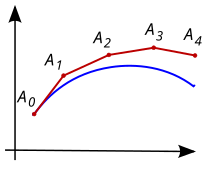
\includegraphics{Euler_method.png}
        \label{Método de Euler}
        \caption{Método de Euler}
    \end{figure}\\
    \vspace{1cm}  
    Dado el problema de valor inicial:\\
        \begin{center}
              $\frac{dy}{dx} = f(x,y)$
            $\hspace*{0.6cm}y(x0) = y0$ 
        \end{center}   
    \vspace{0.5cm}
    El método de Euler con tamaño de paso h consiste en aplicar la fórmula iterativa:
        \begin{center}
             $x_{n+1} = x_n + h$\\
             \vspace*{0.5cm} 
            $y_{n+1} = y_n + h * f(x_n,y_n)$
            \hspace*{0.6cm}$ n\geq 0$\\  
        \end{center}
    \vspace*{1cm}
    La solución de las ecuaciones diferenciales por medio de este método involucra varios tipos de errores:
    \begin{itemize}
        \item \textbf{Error local} : Es la diferencia que se produce entre el valor real de la función y el aproximado mediante la recta tangente suponiendo que el punto desde el que partimos no tiene error alguno.
        \item \textbf{Error acumulado} : Acumulación de errores por las aproximaciones producidas durante los pasos previos acumulados. Es decir, ya no se supone que el punto del cual partimos no tenía error sino que asumimos que dicho error existe y que se propaga de paso en paso. Dicha propagación es, en el peor de los casos, lineal.
        \item \textbf{Error de Redondeo} : Resultado del número límite de cifras significativas que puede retener una computadora. Ya que el número de dígitos utilizados para hacer los cálculos es finito y los números representados puede que no lo sean (es decir, números con infinita cantidad de dígitos). Al limitar los números con infinita cantidad de dígitos (mediante truncamiento o redondeo) a números con finita cantidad de dígitos estamos cometiendo un error extra.
    \end{itemize} 
    Debido a que la aproximación de una curva por medio de una línea recta no es exacta, se comete un error derivado del método. A este error se le conoce como error de truncamiento. Este error se puede disminuir reduciendo el valor de h, pero se obtendrá un mayor número de cálculos y, por consiguiente, un error de redondeo mucho más alto.\\
    Como ya fue explicado anteriormente este método utiliza la pendiente en el punto actual para extrapolar la solución al siguiente punto.
     Esto resulta en un error global de orden \textbf{O(h)} , por lo que para obtener una 
     buena precisión es necesario emplear pasos muy pequeños lo que puede incrementar:
     \begin{itemize}
        \item La cantidad de cálculos y , por ende , el tiempo de cómputo
        \item La acumulación de errores, debido a la limitación de la precisión de la máquina.
     \end{itemize}
    \subsection{Método de Euler Mejorado}
    \vspace*{1cm}
    Ante las limitaciones del Método de Euler surge la necesidad de un método que
    mejore la precisión sin exigir pasos extremadamente pequeños, aumente la estabilidad y minimice la acumulación de errores
    y conserve la simplicidad de implementación en la medida de lo posible. El método de Euler mejorado surge como respuesta a esta necesidad, introduciendo un esquema predictor-corrector.
    La estrategia de este método consiste en realizar una predicción de la pendiente
    $ k_1 = f(x_n,y_n)$. Luego se utiliza el método de Euler para realizar una primera
    estimación de $y_{n+1}$ , a dicha estimación la llamaremos $u_{n+1}$. Ahora que
    se ha calculado $u_{n+1}$ se puede tomar $k_2 = f(x_{n+1},u_{n+1})$ como
    una segunda estimación de la pendiente de la curva solución en $ x = x_{n+1}$.
    Para finalizar se promedian ambas pendientes ($k_1$ y $k_2$) obteniendo así
    una estimación más exacta de la pendiente promedio de la curva solución en 
    todo el subintervalo [$x_n$ , $x_n+1$]\\
    \vspace{1cm}
    \begin{figure}[h]
        \centering
         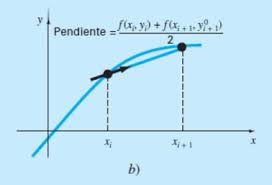
\includegraphics{images.jpeg}
         \label{Euler Mejorado}
         \caption{Método de Euler Mejorado}
    \end{figure}\\
    \vspace{1cm}
    Dado el problema de valor inicial:
    \begin{equation*}
        \begin{aligned}
            \frac{dy}{dx} = f(x,y)
            \hspace*{0.6cm}y(x0) = y0 
        \end{aligned}
    \end{equation*}
    \vspace*{0.5cm}
    El método de Euler Mejorado con tamaño de paso h consiste en aplicar la fórmula iterativa:\\
    \begin{center}
         $ k_1 = f(x_n,y_n)$\\
         $u_{n+1} = y_n + h * k_1$\\
         $k_2 = f(x_{n+1},u_{n+1})$\\
         \vspace*{0.2cm}
         $k = \frac{k_1 + k_2}{2}$\\
         $y_{n+1} = y_n + h * k$\\
    \end{center}
    \textbf{Propiedades:}
    \begin{itemize}
        \item Error global acumulado \textbf{O($h^2$)}
        \item Ventajas:
        \begin{itemize}
            \item Mayor precisión: Permite obtener resultados significativamente más precisos que el método original sin necesidad de reducir demasiado el tamaño del paso.
            \item La corrección basada en la pendiente al final del intervalo disminuye la acumulación de errores.
        \end{itemize}
        \item Desventajas:
        \begin{itemize}
            \item Mayor costo computacional: Se requieren dos evaluaciones de f por cada paso, lo que aumenta el tiempo de cómputo, especialmente en problemas complejos o en sistemas de alta dimensión.
            \item Complejidad de implementación: El algoritmo es algo más complejo, aunque sigue siendo relativamente sencillo en comparación con métodos de orden superior o implícitos.
        \end{itemize}
        \item Aplicaciones: Es ideal en situaciones donde se requiere una mayor precisión en la solución de la EDO, como en simulaciones de fenómenos físicos complejos, modelos de sistemas dinámicos, o en la resolución de problemas en ingeniería y ciencias aplicadas donde el control de errores es crucial.
    \end{itemize}
    \begin{table}[ht]
        \centering
        \begin{tabular}{>{\raggedright\arraybackslash}p{3.5cm}  >{\raggedright\arraybackslash}p{6cm}  >{\raggedright\arraybackslash}p{6cm}}
        \toprule
        \textbf{Característica} & \textbf{Método de Euler Original} & \textbf{Método de Euler Mejorado} \\
        \midrule
        Orden de Precisión & Primer orden (Error global \( O(h) \)) & Segundo orden (Error global \( O(h^2) \)) \\
        \addlinespace
        Evaluaciones de \( f \) por paso & 1 evaluación & 2 evaluaciones \\
        \addlinespace
        Precisión y Acumulación de Error & Menor precisión, requiere pasos pequeños para mayor exactitud & Mayor precisión, menor acumulación de error \\
        \addlinespace
        Costo Computacional & Bajo (rápido y sencillo) & Moderado (aumenta el tiempo de cómputo por paso) \\
        \addlinespace
        Estabilidad & Menor estabilidad en problemas con variaciones rápidas & Mejor estabilidad al promediar las pendientes \\
        \addlinespace
        Complejidad de Implementación & Muy sencilla & Algo más compleja, pero aún accesible \\
        \addlinespace
        Aplicaciones Típicas & Aproximaciones preliminares o problemas simples & Simulaciones donde se requiere mayor precisión y control de errores \\
        \bottomrule
        \end{tabular}
        \caption{Comparación entre el Método de Euler Original y el Método de Euler Mejorado (sin la fila de Fórmula)}
        \label{tab:comparacion}
        \end{table}
        \section{Nueva visita a los números famosos}
        \subsection{Número e}
        \vspace*{1cm}
        $ e \thickapprox 2.71828$ \hspace*{1cm}
        $\frac{dy}{d x} = y$\hspace*{1cm}
        $y(0) = 1$\hspace*{1cm}
        $y(1) = e ??$\\
        \begin{table}[ht]
            \centering
            \begin{tabular}{ccc}
            \toprule
            $n$ & $h$ & $y(1)$ \\
            \midrule
            20   & 0.05    & 2.71719 \\
            40   & 0.025   & 2.71800 \\
            80   & 0.0125  & 2.71821 \\
            160  & 0.00625 & 2.71826 \\
            320  & 0.003125& 2.71828 \\
            \bottomrule
            \end{tabular}
            \caption{Aproximaciones de $y(1)$ para distintos valores de $n$ y $h$.}
            \label{tab:aproximaciones}
            \end{table}\\
        Para aproximadamente n = 320 se logran obtener 5 cifras decimales correctas de e
        \subsection{Número ln2}
        \vspace{1cm}
        $ln2 \thickapprox 0.69315$\hspace*{1cm}
        $\frac{dy}{d x} = \frac{1}{x}$\hspace*{1cm}
        $y(1) = 0$\hspace*{1cm}
        $y(2) = ln2 ??$\\
        \begin{table}[ht]
            \centering
            \begin{tabular}{ccc}
            \toprule
            \(n\) & \(h\) & \(y(2)\) \\
            \midrule
            10   & 0.2    & 0.69563 \\
            20   & 0.1    & 0.69377 \\
            40   & 0.05   & 0.69330 \\
            80   & 0.025  & 0.69319 \\
            160  & 0.0125 & 0.69316 \\
            320  & 0.00625& 0.69315 \\
            \bottomrule
            \end{tabular}
            \caption{Aproximaciones de \(y(1)\) para distintos valores de \(n\) y \(h\).}
            \label{tab:aproximaciones_y1}
            \end{table}\\
            Para aproximadamente n = 320 se logran obtener 5 cifras decimales correctas de ln2
            \subsection{Número $\pi$}
            \vspace*{1cm}
            $\pi \thickapprox 3.14159$\hspace*{1cm}
            $\frac{dy}{d x} = \frac{4}{1+x^2}$\hspace*{1cm}
            $y(0) = 0$\hspace*{1cm}
            $y(1) = \pi ??$\\
            \begin{table}[H]
                \centering
                \begin{tabular}{ccc}
                \toprule
                \(n\) & \(h\) & \(y(1)\) \\
                \midrule
                10   & 0.1     & 3.13993 \\
                20   & 0.05    & 3.14118 \\
                40   & 0.025   & 3.14149 \\
                80   & 0.0125  & 3.14157 \\
                160  & 0.00625 & 3.14157 \\
                320  & 0.003125& 3.14159 \\
                \bottomrule
                \end{tabular}
                \caption{Aproximaciones de \(y(1)\) para el problema correspondiente a \(\pi\) usando el método de Euler mejorado.}
                \label{tab:aproximacion_pi}
            \end{table}
            Para aproximadamente n = 320 se logran obtener 5 cifras decimales correctas de $\pi$
            \section{Investigación de la población logística}
            Dado el problema de valor inicial:\\
            $\frac{d y}{d x} = \frac{1}{3} * y *(8-y) $\hspace*{1cm}
            $y(0) = 1$\hspace*{1cm}
            \begin{table}[ht]
\centering
\begin{tabular}{cc}
\toprule
\(x\) & \(y(x)\) \\
\midrule
10   & 4.3527 \\
20   & 4.3542 \\
30   & 4.3542 \\
40   & 4.3542 \\
50   & 4.3542 \\
60   & 4.3542 \\
70   & 4.3542 \\
80   & 4.3542 \\
90   & 4.3542 \\
100  & 4.3542 \\
\bottomrule
\end{tabular}
\caption{Tabla para demostrar el estancamiento de la solución en 4.352}
\label{tab:euler_mejorado}
\end{table}\\
Analicemos problema de valor inicial:\\
   $\frac{dy}{dx} = \frac{1}{n} * y * (m-y) $\hspace*{1cm}
   $y(0) = 1$\\
   \vspace{0.5cm}
   Supongamos que n = 2 y m = 1\\
   Esta ecuación la podemos resolver de forma analítica mediante la resolución
   por Variables Separadas estudiada en clases. Llegando a que la función solución es:\\
   $y(x) = \frac{e ^ \frac{x}{2} }{1 + e^\frac{x}{2} }$\\
   Dicha función tiende a uno por lo que podemos garantizar que este es
   el límite ¨correcto¨.\\
   A continuación se analizará que tanto se acerca el método de Euler Mejorado
   para un tamaño de paso de 1 a dicho límite
   \begin{table}[H]
    \centering
    \begin{tabular}{cc}
    \toprule
    \(x\) & \(y(x)\) \\
    \midrule
    10   & 1.0 \\
    20   & 1.0 \\
    30   & 1.0 \\
    40   & 1.0 \\
    50   & 1.0 \\
    60   & 1.0 \\
    70   & 1.0 \\
    80   & 1.0 \\
    90   & 1.0 \\
    100  & 1.0 \\
    \bottomrule
    \end{tabular}
    \caption{Tabla que muestra el acercamiento de Euler Mejorado a la solución "real" de la ecuación}
    \label{tab:euler_mejorado}
    \end{table}
    En este caso para h = 1 obtuvimos un aproximación muy cercana
    a la solución ¨real¨ pero podemos decir que generalmente este no nos
    llevará a una aproximación muy precisa del valor límite m , por lo que
    en gran parte de los casos se requerirá de una reducción en el tamaño de h
\end{document}